\documentclass[12pt]{article}
\usepackage{graphicx}
\title{Reto 02\\Modelado y Programaci\'on\\José de Jesus Galaviz Casas}
\author{Uriel Garc\'ia Luna Bobadilla y Mauricio Riva Palacio Orozco}
\date{}
\begin{document}
    \maketitle
    \begin{enumerate}
        \item Definici\'on del problema:\\  Crear un programa con interfaz gr\'afica que cargue im\'agenes, las muestre y sea capaz de aplicarle 4 filtros distintos modificando sus pixeles: rojo, azul, verde y mosaico.
        \item An\'alisis del problema:\\Primero se debe  de buscar un lenguaje en cual no sea demasiado complicado o tardado desarollar una interfaz gráfica como \textsl{Java} o \textsl{Pyhton} para que no se gaste tiempo excesivo en el desarrollo de \'esta.\\De igual manera se debe buscar un lenguaje que facilite el manejo de imágenes y pixeles con algún objeto en su biblioteca.
        \item Selecci\'on de alternativa:\\Se decidi\'o hacer la interfaz gr\'afica usando \textsl{HTML5} y \textsl{CSS3} pues es la forma m\'as facil de hacerla adem\'as tambi\'en se consider\'o que ser\'ia lo m\'as c\'omodo para el usuario pues para correr el programa no necesitar\'a mas que un navegador web.\\ Para la parte de los filtros (que es la parte de c\'odigo) el lenguaje seleccionado fue \textsl{JavaScript} por su compatibilidad con \textsl{HTML5} adem\'as de que tiene el objeto \textit{canvas} el cual al brinadarle un archivo de imagen nos permite desplegarla facilmente y acceder a sus pixeles para la modificaci\'on de \'esta.\\ Por la forma en la que trabaja \textsl{JavaScript} (o al menos con la cual nos percatamos en el equipo siendo que nunca hab\'iamos programado en este lenguaje) no se creo ninguna clase, todo es funcional y los algoritmos solo se ejecutar\'an cuando sean llamados por los inputs a los que esten vinculados, tambien nos percatamos que gracias a canvas aplicar los filtros: rojo, azul y verde es el mismo c\'odigo solo que con diferentes valores a aplicar en cada imagen, es por esto que el aplicar filtro es solo un m\'etodo que aplicar\'a siempre los valores de un arreglo, los valores del arreglo se cambiar\'an seg\'un el color del filtro que selecione el usuario; el \'unico filtro en el que cambiar\'a la aplicaci\'on ser\'a el de mosaico, sin embargo al ser solo un cambio se dej\'o en la misma funci\'on separado por un \textit{if}.
        \item Diagrama de flujo: \\ 
        \begin{figure}[h]
            \centering
            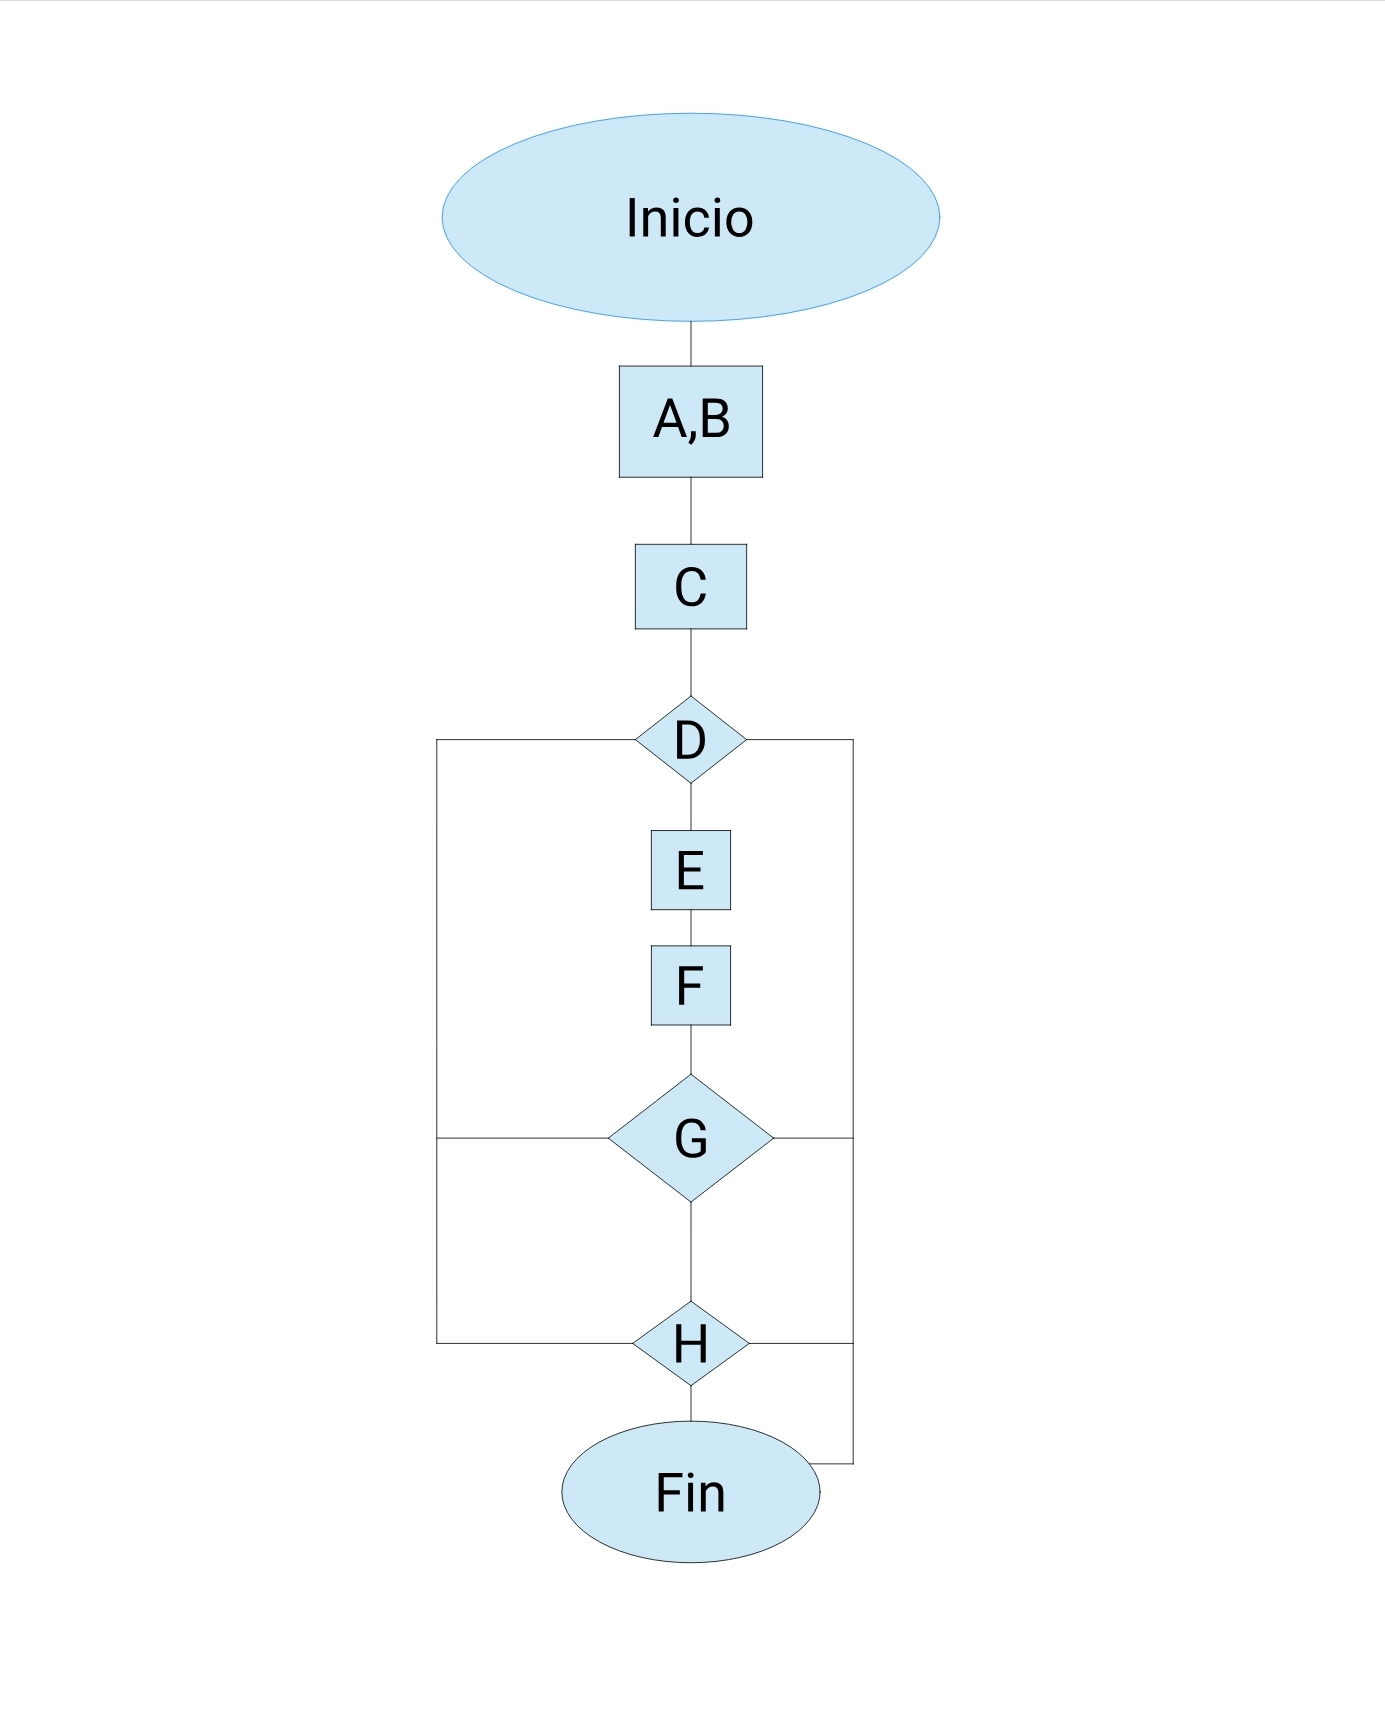
\includegraphics[height = 10cm ]{Diagrama.jpg}
        \end{figure}
        \\Este programa no sigue un orden secuencial estricto por estar hecho en \textsl{HTML5} y \textsl{JavaScript} el usuario puede hacer las acciones que guste en el orden que guste sin embargo esta es la secuencia de pasos(junto con las acciones que desencadenan estos )que debe seguir para el correcto funcionamiento del programa :\\ 
        A: recibir tipo de filtro, B: recibir archivo, C: procesar el archivo, D: el archivo es  una imagen, E: insertar imagen en canvas, F: aplicar filtro a imagen, G: borrar el filtro actual, H: borrar imagen actual\\
        Las letras que aparecen en un mismo cuadro representa que no importa el orden de estas y cualquiera puede pasar antes que la otra.\\
        El programa no tiene como tal un "fin" ya que el usuario puede cambiar de imagen y de filtro cuantas veces quiera y termina cuando el cierra la p\'agina, solo se pone en el diagr\'ama para representar cuando ya no hay mas acciones posibles en el programa.
        \item Descripci\'on del trabajo:\\ En este trabajo al ver que no habr\'ia una clase por filtro por lo explicado en el punto 3 un integrante hizo los filtros: rojo, azul y verde , mientras que el otro integrante realiz\'o el del filtro mosaico; para el resto del trabajo un integrante realiz\'o la interfaz gr\'afica con todos los metodos que \'esta deb\'ia incluir y el archivo pdf mientras que el otro integrante realiz\'o los test y el README.
        \item Mantenimiento a futuro:\\El programa puede tener varios cambios como el que se muestren varias im\'agenes al mismo tiempo, nuevos filtros y mejora de diseño, entre algunos otros.\\El precio que se cobrar\'ia por este programa ser\'ia de 1300 pesos mexicanos aproximadamente y de 300-400 pesos mexicanos seg\'un sea el caso.
\end{document}
